\documentclass[]{article}

\usepackage[utf8]{inputenc}

\usepackage{eurosym}
\usepackage[
  margin=1.8cm,
  includefoot,
  footskip=10pt,
]{geometry}
\usepackage{graphicx}
\graphicspath{{figures/}}
\usepackage[english]{babel}
\usepackage{url}
\usepackage[colorlinks=true, linkcolor=black, urlcolor=blue]{hyperref}
\usepackage{color}
\usepackage[dvipsnames]{xcolor}
\usepackage{titling}
\usepackage{subfig}
\usepackage[bottom]{footmisc}
\usepackage{titlesec}
\usepackage{chngpage}
\usepackage{calc}
\usepackage{listings}

\definecolor{gray}{rgb}{0.4,0.4,0.4}
\definecolor{darkblue}{rgb}{0.0,0.0,0.6}
\definecolor{cyan}{rgb}{0.0,0.6,0.6}

\lstset{
  basicstyle=\ttfamily,
  columns=fullflexible,
  showstringspaces=false,
  commentstyle=\color{gray}\upshape
}


\setcounter{secnumdepth}{4}


\newcommand{\minit}[1]{\noindent{\small\textbf{ \underline{#1}}}~\\}
\newcommand{\todo}[1]{\par{\color{red} /---| A faire : #1 |---\textbackslash\\}}
\newcommand{\todoIL}[1]{{\color{red}[todo: #1]}}
\newcommand{\wordlink}[2]{\hyperref[#2]{#1~\ref{#2}}}

\titleformat{\paragraph}
{\normalfont\normalsize\bfseries}{\theparagraph}{1em}{}
\titlespacing*{\paragraph}
{0pt}{3.25ex plus 1ex minus .2ex}{1.5ex plus .2ex}

%-- Logos PDG --
\pretitle{
\begin{center}

\begin{figure}[!tbp]
  \centering
  \subfloat{
\includegraphics[width=0.25\textwidth]{UMons_logo.png}}
  \hfill
  \subfloat{
\includegraphics[width=0.25\textwidth]{sciences_logo.png}}\\
\end{figure}
~\newline

}

\posttitle{\end{center}}

\begin{document}

\title{
\vspace{1.6cm}
{\Huge Software Analysis : pacman systems}\\
\vspace{0.5cm}
{\Huge Project report for Software Evolution course}\vspace{1cm}\\
}


\author{
\vspace{1cm}
\huge{Group 3}\\
\Large{BOOSKO Sam}\\
\Large{DECOCQ Rémy}\\
\Large{SCHERER Robin}
}


\date{
\vspace{7.9cm}
Academic Year 2019-2020\\
Master Computers Science, block 2\\
Faculté des Sciences, Université de Mons}

\maketitle          

\thispagestyle{empty}   

\newpage

\tableofcontents
\newpage

%------------- INTRO -------------
\section*{Introduction}
\newpage
\section{Quality analysis of the initial versions}
\label{quality_analysis}

\subsection{System 2 (Rémy)}
\subsubsection{Generalities}

First of all, this is noticeable that authors provide some documents coupled with the implementation, even if it is not mentioned in the README file. This additional material is available under the \texttt{out/} directory at project roots and comprises :
\vspace{0.1cm}
\begin{itemize}
\item A \texttt{.pdf} file describing shortly the game, the controls and the multiplayer (2 players) mode available

\item A complete class diagram covering the whole implementation

\item A sequence diagram stating the execution flow when Pacman arrives on a cell and so ``eat" what is at this place

\item A graph of the mathematical function used to correlate difficulty with player's progression
\end{itemize}

We also observe that in this Pacman implementation maps are modelized under \texttt{.tmx} format, that is a popular way to deal with board games\footnote{\url{https://doc.mapeditor.org/en/stable/reference/support-for-tmx-maps/}}. Only one single basic map is provided.\\

The project structure is classic, we have \texttt{main} and \texttt{test} separation under the \texttt{src} directory, each containing packaged sources. The building system provided with the implementation is hold by Gradle. So a switch to Maven will be required to comply with directives.


\subsubsection{Static Analysis}

\paragraph{Code metrics (CodeMR)}

CodeMR allows to get an overall idea of the actual health of the system considering several metrics. The dashboard illustrated by \wordlink{Figure}{fig:S2_codeMR_dashboard} informs this software is doing quite good.

\begin{figure}[h]
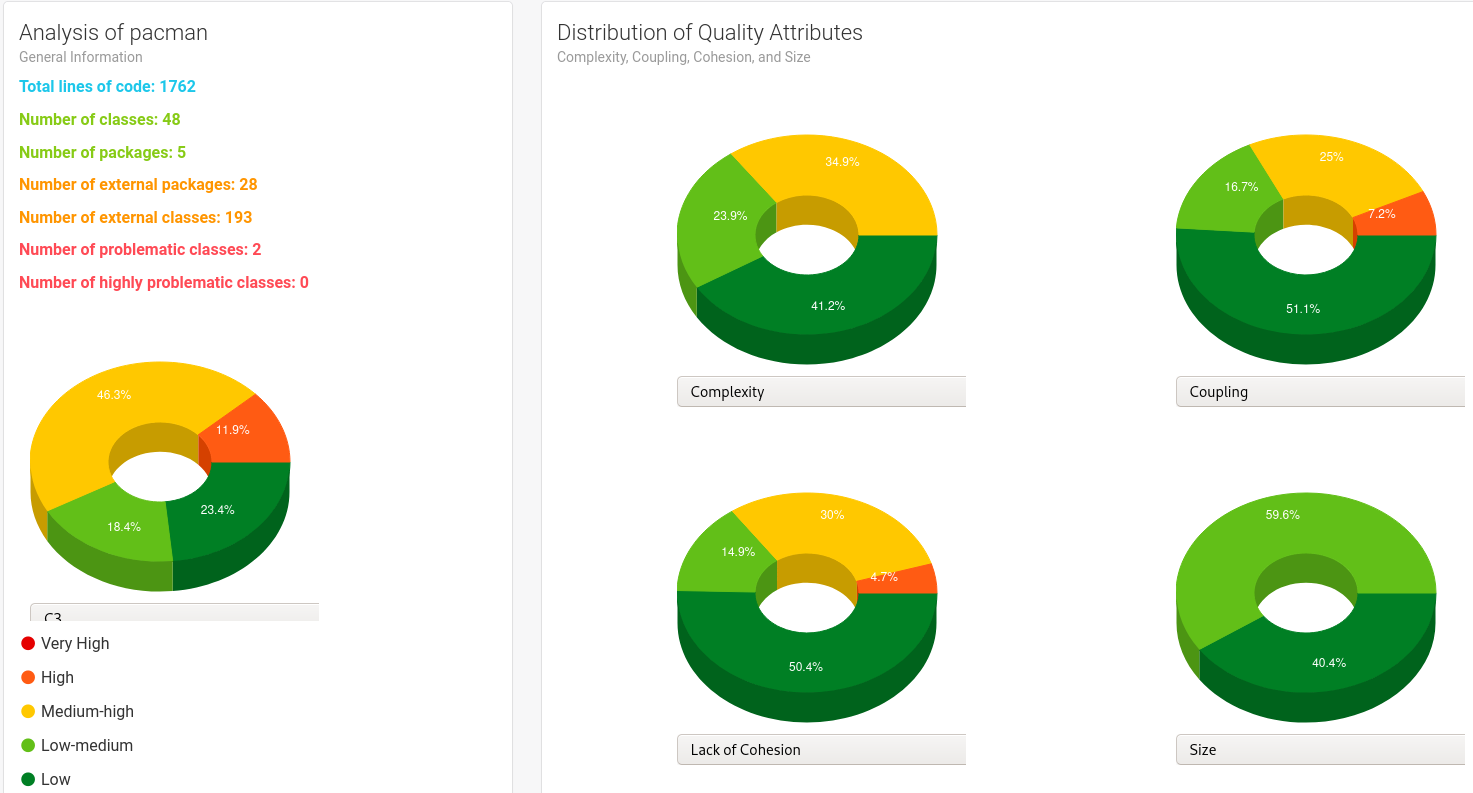
\includegraphics[width=\linewidth]{S2-codeMR_dashboard}
\caption{CodeMR dashboard summarizing health of system 2}
\label{fig:S2_codeMR_dashboard}
\end{figure}

\newpage

The \wordlink{Figure}{fig:S2_codeMR_packages} illustrates also the C3 metric but coupled with detailed packages view. We notice authors apparently tried to follow some Model-View-Controller pattern to design their application. The C3 metric is defined as the maximum between 3 other well representative metrics : \textit{Coupling}, \textit{Cohesion} and \textit{Complexity}. These are defined in the codeMR documentation\footnote{\url{https://www.codemr.co.uk/documents}}. We notice that, following the dashboard overview, two classes are impacting the software quality from the point of view of C3 metric.
\vspace{0.2cm}
\begin{figure}[h]
\centering
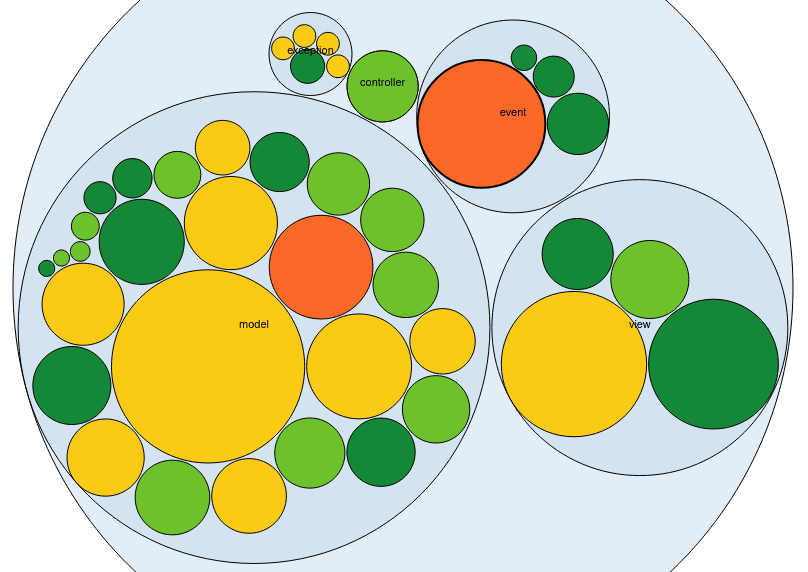
\includegraphics[width=0.8\linewidth]{S2-codeMR_packages}
\caption{C3 Metric by package for system 2}
\label{fig:S2_codeMR_packages}
\end{figure}

The details of the measurements on the two more problematic classes are given by \wordlink{Figure}{fig:S2_workerProcess} and \wordlink{Figure}{fig:S2_ghost}, for respectively \textit{event.WorkerProcess} and \textit{model.Ghost}. For both, two metrics are considered as high value, the meaning described by CodeMR is
\begin{itemize}
\item LTCC : The Lack of Tight Class Cohesion metric measures the lack cohesion between the public methods of a class. That is the relative number of directly connected public methods in the class. Classes having a high lack of cohesion indicate errors in the design.
\item LCOM : Measure how methods of a class are related to each other. Low cohesion means that the class implements more than one responsibility. A change request by either a bug or a new feature, on one of these responsibilities will result change of that class. Lack of cohesion also influences understandability and implies classes should probably be split into two or more subclasses.
\end{itemize}

In addition, for \textit{event.WorkerProcess} we have :
\begin{itemize}
\item CBO : The number of classes that a class is coupled to. It is calculated by counting other classes whose attributes or methods are used by a class, plus those that use the attributes or methods of the given class.
\item AFTD : Access to Foreign Data is the number of classes whose attributes are directly or indirectly reachable from the investiggated class. Classes with a high ATFD value rely strongly on data of other classes and that can be the sign of the God Class.
\end{itemize}

Other codeMR metrics did not revelate relevant problems in the implementation.

\newpage

\begin{figure}[h]
\centering
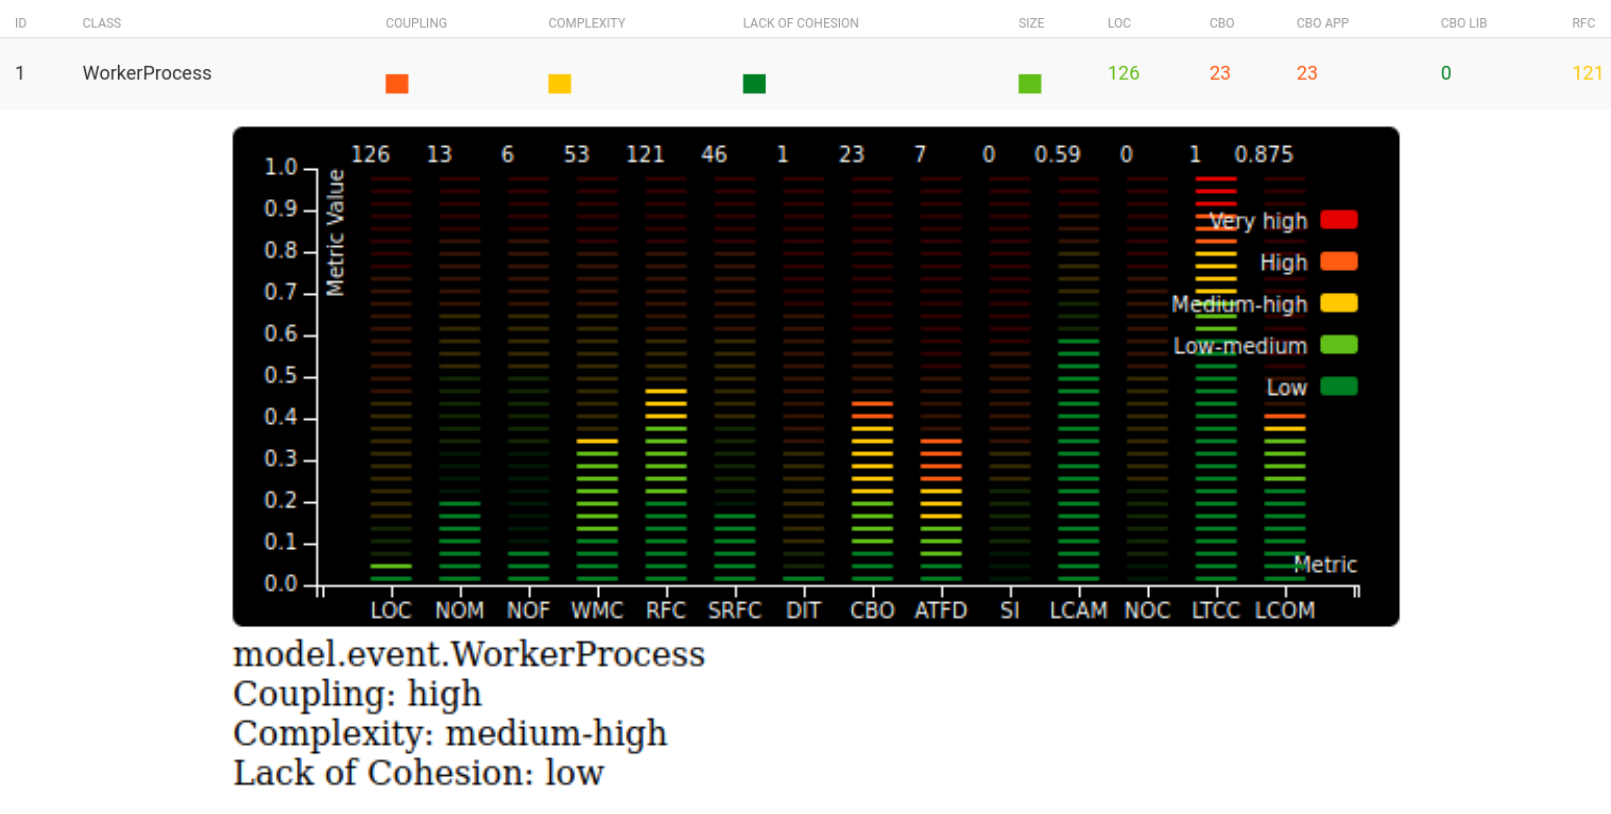
\includegraphics[width=0.9\linewidth]{S2-WorkerProcess_full}
\caption{\textit{event.WorkerProcess} class main metrics measurements}
\label{fig:S2_workerProcess}
\end{figure}

\begin{figure}[h]
\centering
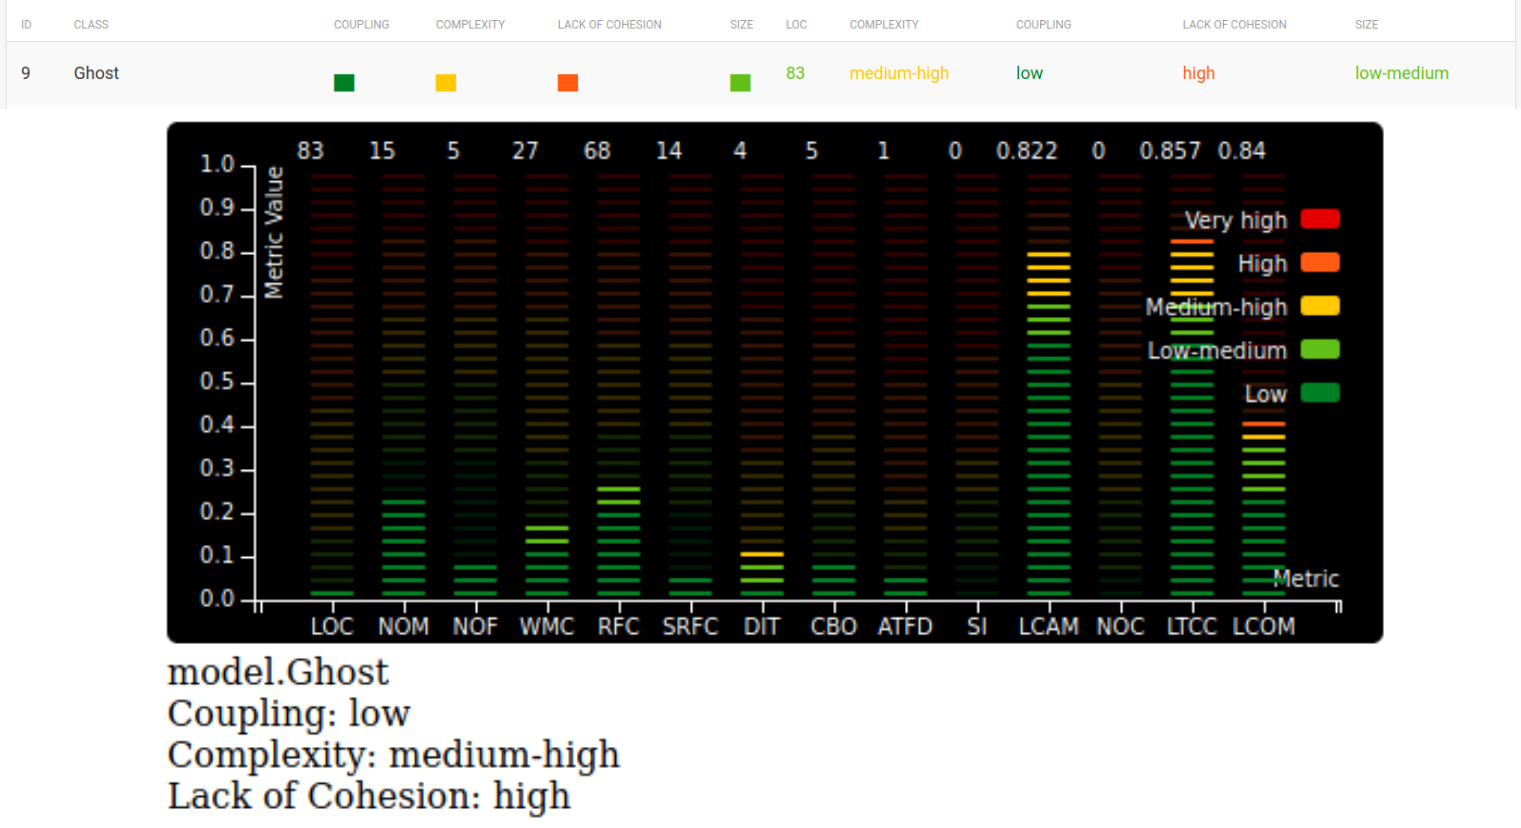
\includegraphics[width=0.82\linewidth]{S2-Ghost_full}
\caption{\textit{model.Ghost} class main metrics measurements}
\label{fig:S2_ghost}
\end{figure}
  
\newpage

\paragraph{Dependencies (CodeMR, Intellij analyzer)}

CodeMR allows also to inspect dependency relations between classes coupled with the metrics measured for each. We observe in the \wordlink{Figure}{fig:S2_inheritance} the same structure that in the class diagram. Once again the class \textit{event.WorkerProcess} is displayed as problematic, being too complex and coupled with other classes.\\

We use the standard built-in tool of IntellIJ IDEA to instantiate the dependency matrix, illustrated by \wordlink{Figure}{fig:S2_dep_matrix}. We clearly see reading 8th column that \textit{event.WorkerProcess} depends on a lot of other classes from package \textit{model}. This is also the case for \textit{model.Map} that presents a lot of cyclic dependencies (red marked).

\paragraph{Compliance \& bad smells (PMD, Designite)}

PMD is a statical analyzer that checks for problems of several natures in the code. It detected more than 1500 violations in the system 2, related to various topics (see \wordlink{Figure}{fig:S2_PMD}).

\vspace{0.3cm}

\begin{figure}[h]
\centering
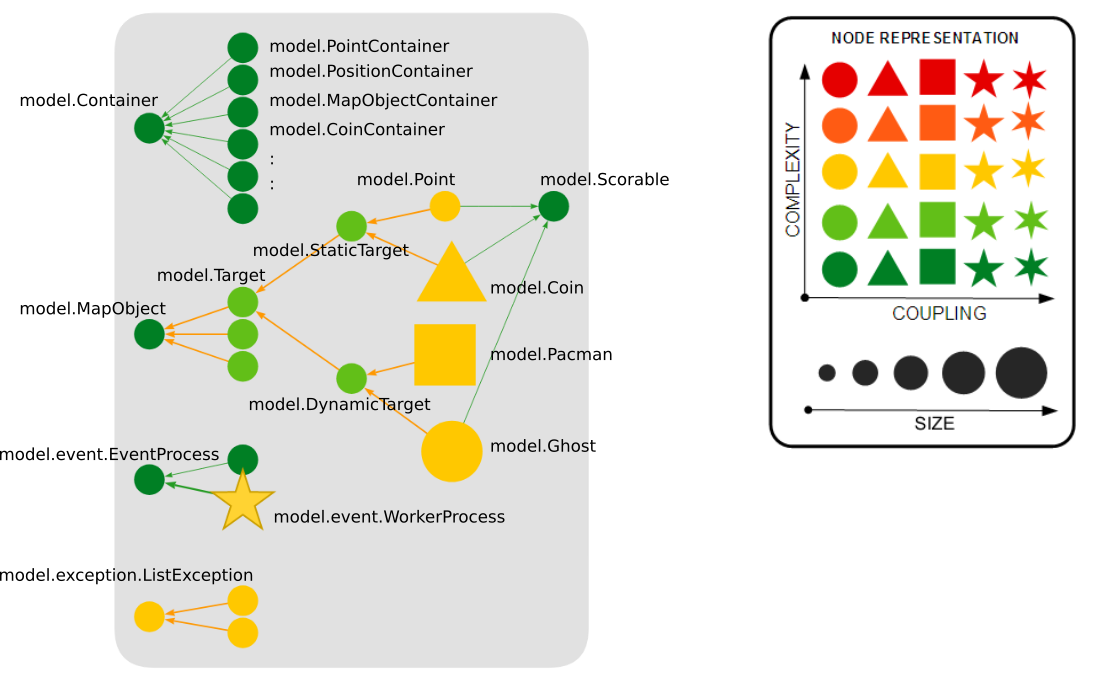
\includegraphics[width=0.8\linewidth]{S2-named_inheritance}
\caption{Inheritance relations between classes in system 2}
\label{fig:S2_inheritance}
\end{figure}

\vspace{0.4cm}

\begin{figure}[h]
\centering
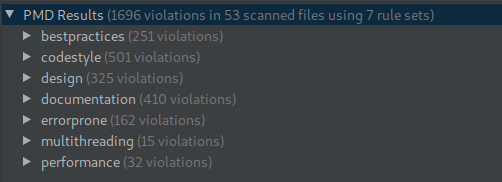
\includegraphics[width=0.7\linewidth]{S2-PMD_results}
\caption{Violations found by PMD in system 2}
\label{fig:S2_PMD}
\end{figure}

\newpage

\begin{figure}[h]
\centering
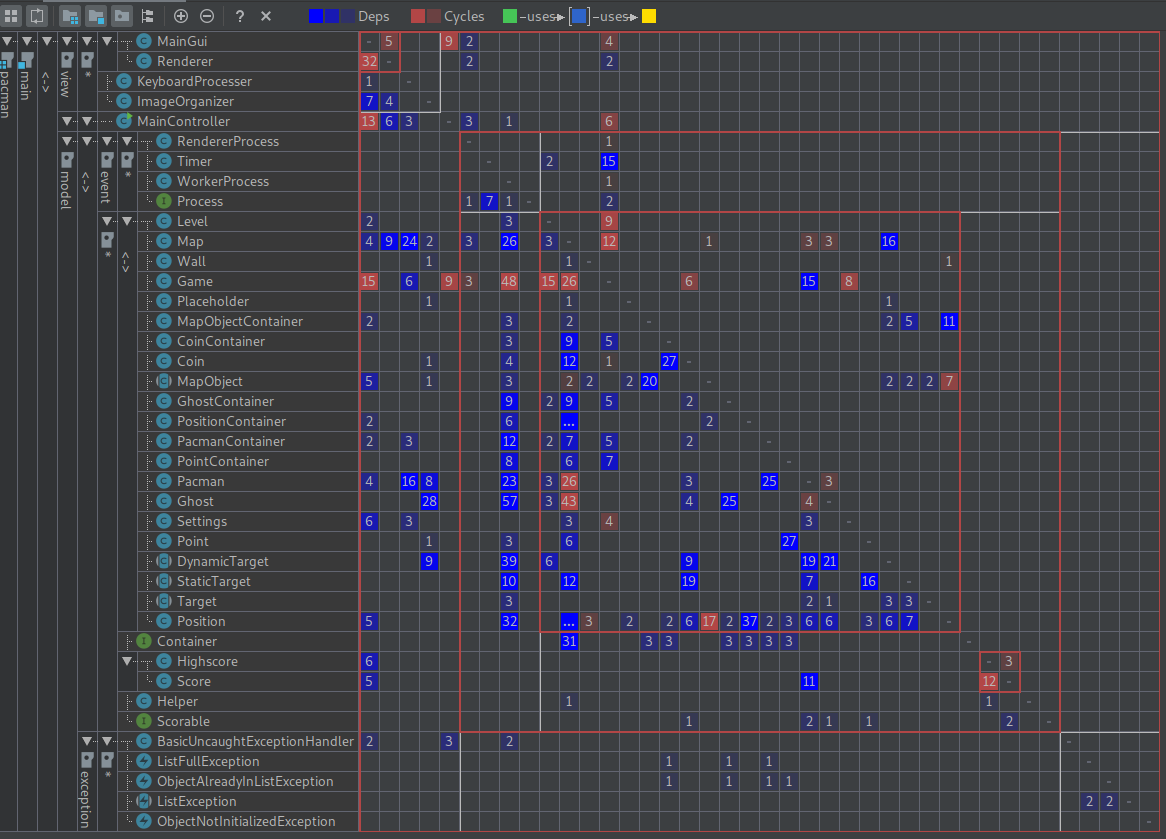
\includegraphics[width=0.9\linewidth]{S2-dep_matrix}
\caption{Dependency matrix for system 2}
\label{fig:S2_dep_matrix}
\end{figure}

\vspace{0.1cm}

Designite is used to detect bad smells, a summary of the analyse is presented by \wordlink{Figure}{fig:S2_designite}. The number of lines of code and classes is higher than the ones returned by CodeMR because the test sources were considered in the analysis.

\begin{figure}[h]
\centering
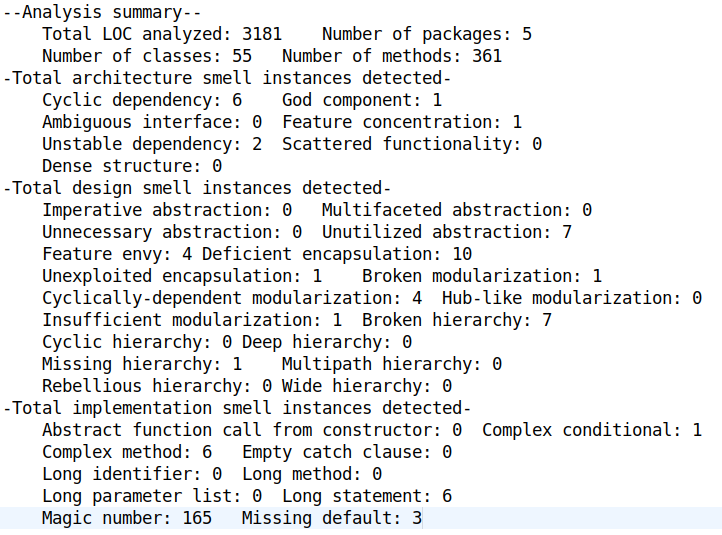
\includegraphics[width=0.65\linewidth]{S2-designite}
\caption{Designite in-line use results for system 2}
\label{fig:S2_designite}
\end{figure}


\newpage


\paragraph{Javadoc coverage (MetricsReloaded)}

We use the IntellIJ MetricsReloaded plugin and its metric "Javadoc coverage" to get an overview of how complete is the initial javadoc. As shown by \wordlink{Figure}{}, this is the case.

\vspace{0.2cm}

\begin{figure}[h]
\centering
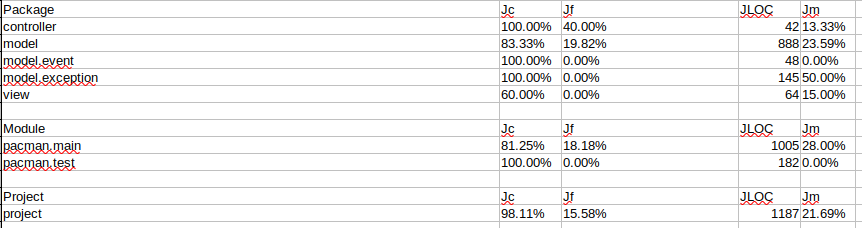
\includegraphics[width=0.65\linewidth]{S2-javadoc}
\caption{Javadoc coverage for system 2}
\label{fig:S2_javadoc}
\end{figure}

\subsubsection{Dynamic Analysis}

\paragraph{Running tests}

Among the already written tests, 3 out of 67 failed at running time. The three tests are in \textit{model.LevelTest} (\textit{testGetLevel}, \textit{testSecondsForCoin} and \textit{testNextLevel}). 

\paragraph{Test coverage (Intellij built-in tool)}

IntellIJ provides run configurations to dynamically analyze what are the parts of source codes covered by launched tests. Considering whole test packages, summary of the results are given by \wordlink{Figure}{fig:S2_test_coverage}. We observe the implementation benefits of a good test coverage, the most laking part is package \textit{view} but it makes sense by its nature.

\newpage

\begin{figure}[h]
\centering
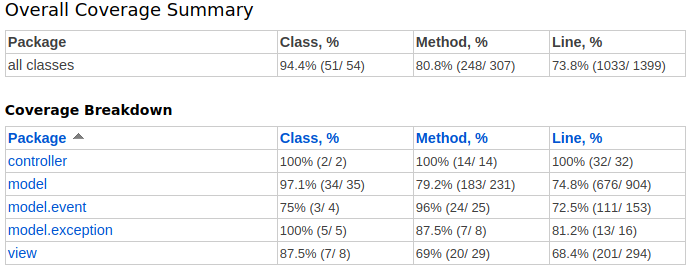
\includegraphics[width=0.75\linewidth]{S2-test_coverage}
\caption{Test coverage for system 2}
\label{fig:S2_test_coverage}
\end{figure}

\newpage
\section{Quality improvement}

\subsection{System 2 (Rémy)}

We employ the following methodology to improve the system in its current state :
\begin{enumerate}
\item Reviewing the whole code and correct problems of form. It allows to acquire a global overview of the implementation to lead next steps and improve code quality on a per-class basis. These refractorings comprise, among others :
\begin{itemize}
\item completing the Javadoc
\item getting rid of forgot/useless artifacts
\item detecting and correcting code smells
\end{itemize}
The main tool used during this step will be the IDE (IntellIJ) and plugins associated with like Designite, which allow on-the-fly analysis and pointing out problems in the code itself.


\item Reviewing the system structure and correct structural design problems. From the acquired global overview, it is possible to have an idea of drawbacks implied by the system design. The refractoring will occurr at a class-to-class relations level, and will then impact package structure level. Some tools and metrics, for example from CodeMR, can be used to leas this step : a class reported too long may be splitted into more than 1 class, inheritance should be used better, etc.

\item If some tests are not passing, find the reason and correct them.

\item Complete the tests based on test coverage reports generated (from IntellIJ).
 
\end{enumerate}
\vspace{0.2cm}
Of course, after each of these steps, the current yet written tests must be launched to control the consistence of the implementation.

\subsubsection{Step 1}

\indent\par We read through the whole code and corrected what had to be in a first time. Some smells are straightforward, like avoiding Magic Numbers detected by Designite. The help of IntellIJ is precious to get rid of some deprecated/forgot code artifacts the authors left. Some problems reported by Designite are not regarding the actual usage and left as-is.

\subsubsection{Step 2}

\indent\par It was figured out the current implementation presents some drawbacks. It is mainly related to code duplication for already written objects for \texttt{Container} purposes (can be found in provided class diagram). The fact is that authors wanted to write an overlayer to describe different collections of other objects in the implementation (\texttt{Coin} (= pills), \texttt{Point}, etc.). But they wrote a specific class for every type of object to contain, albeit implementing the common \texttt{Container} interface, this design is very poor and ineleguant, leading to code duplication and increased number of classes. Keeping in mind what were each class written for, we redisigned this part of the implementation in a better way. It also brought the occasion to cluster \texttt{Container} class concerned in a new package to improve the project structure readability.\\

The resulting structure is depicted by \wordlink{Figure}{fig:S2_containers}. We now consider to pass through a \texttt{Containers} class to construct any \texttt{Container} needed in the rest of the implementation. Its static methods instantiate the right container with adapted type of content from generic classes. These instances are shown in orange in the \wordlink{Figure}{fig:S2_containers}. The restricted typing \texttt{E extends MapObject} allows getting element(s) considering a \texttt{Position} object. A \texttt{PositionContainer} is a specialized container to hold coordinates (already present in original code), so we dont use an index but form a key from the couple ($x$, $y$). The method \texttt{getRange(..)} allows to get a subset of contained positions, considering a rectangle selection formed from two positions given in parameters. For some object types (\texttt{Point}), an overload is necessary to comply with the rest of the implementation. Anyway, this is somehow masked because all containers instances are retrieved from the class \texttt{Containers} mentioned above,  not represented in the figure.

\newpage

\begin{figure}[h]
\centering
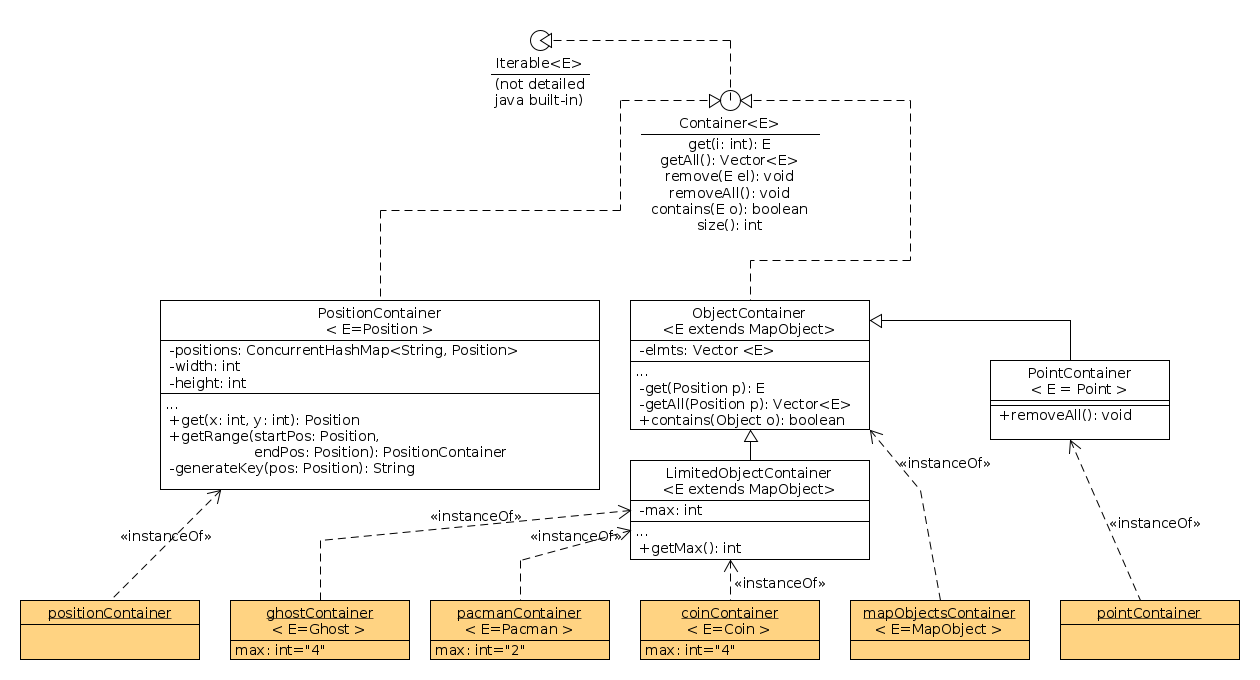
\includegraphics[width=\linewidth]{S2-classdiagram_containers}
\caption{New class structure for \texttt{Container}s part of the implementation}
\label{fig:S2_containers}
\end{figure}


An other problem is related to the \texttt{Map} class. We observe the Map itself and the objects that will represent it in the application are instantiated in raw. Coordinates for each element are given in the code itself, that is a bad practice. However, due to the lack of time and considering the picked extension doesn't relate to maps, a trade-off is taken. A new class \texttt{MapPlacer} is written to hold the placement of \texttt{MapObjects} on the declared possible \texttt{Positions} of the unique considered map. It cleans up the code of the original class \texttt{Map} that should only hold dynamic operations such as reinitializing the content of the map when the player passes a level.\\

Concerning package structure, some changements were also needed because the \texttt{model} package had no sub-level (grouping almost 30 classes). We added a subpackage \texttt{model.container} that holds all the hierarchy depicted above and another \texttt{model.mapobject} to group all classes standing for the actors/components of the game (\texttt{Wall}, \texttt{Pacman}, \texttt{Coin}, etc.).

\subsubsection{Step 3}

\indent Some already written tests were not passing, or passing but throwing an exception. That was mainly due to the management of multithreading and game reseting not properly. Also, the usage of \texttt{static} elements lead to inconsistencies. Leveraging some adjustements in the source code, we managed to get the system more consistent and the tests passing in a determenistic behaviour.

\subsubsection{Step 4}

\indent \par The provided existing tests are numerous but not relevant for some. Firstly, there are empty tests, whose only signature is written. They were filled in the right way to evaluate what they're expected to. Some others focus only on get/accessors and methods that are even never used in the rest of the implementation. So, tests oriented to behavior evaluation are mainly missing. We added some for \texttt{Map}, \texttt{Ghost}, \texttt{Pacman}, etc. They aim to ensure the game is running as expected. More diverse additions were done all over to improving testing quality.\\

As some new classes have been written to improve the system quality, the associated tests were also written. We have \texttt{PositionContainerTest} and \texttt{TimerTest} to evaluate the new implementation parts described above.

\newpage
\section{Adding basic functionalities}

\subsection{System 2}

The following functionnalities were pointed out as missing in this system :

\begin{itemize}
\item The last two pills eaten in a Level must give an invicibility of 5 seconds instead of 7 seconds
\item A ghost must disappear when munched and respawn in the ghost base after 5 seconds
\item Consecutive eaten ghosts must give more points (200-400-800-1600)
\item There is a timer ruling each level (stoped when pacman is hunting)
\end{itemize}

\vspace{0.2cm}

The commit corresponding to the final version of the basic game is \\

\url{https://github.com/RemDec/pacman-system2/commit/cb5e36143d6ab84a9c02d80cd4c58ae56ff0e8aa}

 ~\\

These functionnalities are somehow straightforward to implement in this system. Of course some unit tests are written to verify the new behaviors. The only remark would go to the timer. As this system is intended to strengthen the difficulty increasing the ``refresh rate", this rate govern the display frequence. This is why the displayed timer increments step-by-step (we avoid using new display threads to keep consistency and good integration in the actual system). As this timer feature was not present, new classes \texttt{Timer} and \texttt{TimerProcess} were written to be easily integrated with the already existing \texttt{Scheduler} (renamed, previously \texttt{Timer}). The timer has been integrated to the interface as depicted by \wordlink{Figure}{fig:S2_timer}.\\

It was also necessary to correct some hidden bugs related to the behavior of ghosts. Sometime when eaten, they stay at their position instead of respawning in their base. The code was modified to obtain the right behavior and some tests were added to ensure this. \\


\begin{figure}[h]
\centering
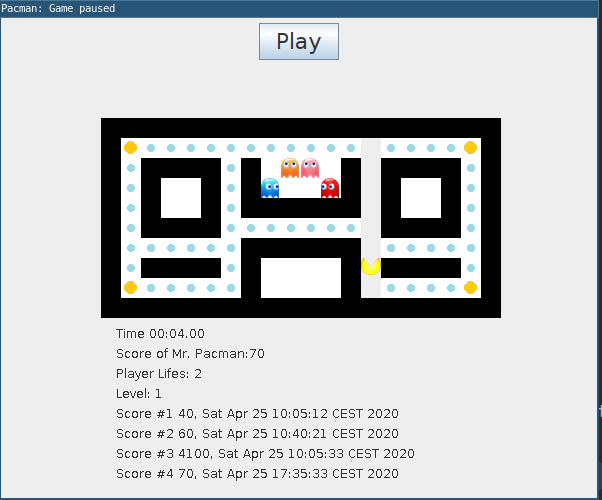
\includegraphics[width=0.6\linewidth]{S2-screen_timer}
\caption{New timer integrated in the interface (below the map)}
\label{fig:S2_timer}
\end{figure}

\newpage
\section{Adding new features}

\subsection{System 1 (Rémy)}

\subsubsection{New features discussion}

\indent\par The integration of special fruits/boxes in this system is quite facilitated by the quality of the implementation, which allows to define new unities and their collision map in a generic way. It is done by subclassing \texttt{Unity} class or one of its already existing subclasses. For example, for new fruits that apply an effect within a given duration, a generic class \texttt{SpecialPellet} is written, extending \texttt{Pellet}. It handles the duration and resetting original state once exhausted. Each fruit is a short subclass of it (\texttt{PotatoPellet} for example) which implements its logic depending the associated effect. We managed to give a variation in each effect that makes sense with the current game state. For \texttt{PotatoPellet}, the more pacman has score, the juicier he looks for ghost so they are buffered for an increased duration. Note that we made the choice that duration effects are not cumulutative to keep the game clear and the current Pacman state always indicated to the player (thanks to the Pacman's skin). Though Pacman can still become a hunter during a special effect (indicated by ghosts skin).\\

Implementing special boxes is also somehow straightforward : we sublcassed \texttt{Unity} with \texttt{SpecialBox} and each box is a subclass of the latter. These boxes have an impact on the game logic and are not especially coupled with a duration. It lead to modifications on the collisions logic. For instance, \texttt{BridgeBox} implements bridges that required an introduction of the vertical level notion (\texttt{DOWN} and \texttt{UP}), a state associated with each unit. We reconsidered collisions to be handled occurring only between units in the same vertical level.\\

The detail about each special unit and the way effects vary depending current game state can be found in the corresponding class documentation. An illustration of the implemented special units is provided by \wordlink{Figure}{fig:S1_special} (illustrating actual effect is quite difficult for most, it should be played instead).\\


\begin{figure}[h]
\centering
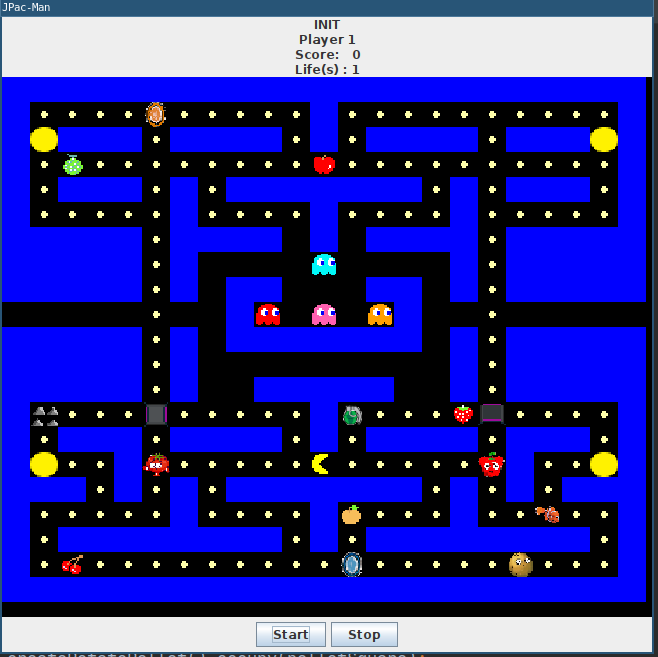
\includegraphics[width=0.62\linewidth]{S2-extension}
\caption{Illustrating all special units on the bottom of the map}
\label{fig:S1_special}
\end{figure}

\newpage

Apart from the effect of special units, it was also asked to make them dynamically spawn taking account the current state of the level. This new mechanic is handled by the class \texttt{SpecialUnitySpawner}. At a fixed time interval (7 seconds), a try is done to spawn a special unit on the board : this decision is made in a probabilistic fashion. The process accounts for the following guidelines :
\begin{itemize}
\item if the board is nearly empty (ie. there are a few pellets compared to the number initially present), it could be good to fill it a bit to change the destiny of this game that seems nearly over. So chances to spawn a new unit are higher in this configuration (exact formula in code).
\item as pellets are eatable, that is not the case for boxes that are persistent. To avoid overloading the board, we set a probability to choose a pellet at 0.7.
\item in the case of a pellet to spawn, we have possible bonuses and penalties. The decision is made looking to the current player score. The higher it is, the closer he should be to the win and it also indicates the player is good. So we make his job harder, giving more probability to spawn a penalty pellet.
\item the decision of which box/pellet will spawn among available is uniformally random.
\end{itemize}

\vspace{0.4cm}

Finally, we restructured the packages for special units to group pellets and boxes. The final commit, with a playable and balanced game and all tests passing is accessible here :\\~\\
\url{https://github.com/Lroemon/pacman-system1/commit/e7a404331bb5577c5e8d6145059f7c6379b029e5}

\subsubsection{Quality analysis}

\indent From the extension development point of view, this implementation was really nice and easy to extend. The code was already well documented, and all is structured in a way it is quickly understandable. As the quality analysis at the beginning of the project mentionned, this is a quite good implementation that suffers really few drawbacks.
We lead firstly some statis analysis to get an overview of how the implementation evolved. 


\begin{figure}[h]
\centering
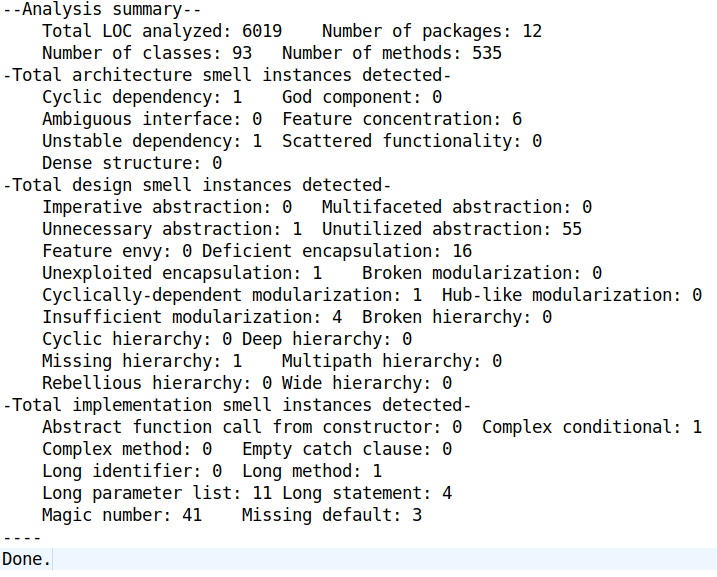
\includegraphics[width=0.7\linewidth]{S1-designite_final}
\caption{Results from Designite for final system 2}
\label{fig:S1_designite_final}
\end{figure}

\newpage

We observe in \wordlink{Figure}{fig:S1_designite_final} that the system has consequently increased in size, almost doubled in mulitple counting metrics (LOC, number of classes/methods). The increasing size of the code lead to some new bad smells, but also avoided some previously present. Some metrics like magic numbers seem still (41 now, 39 previously), but actually this is not the case considering the implementation almost doubled in size. An metric that increased a lot is the unutulized abstraction, growing from 4 to 55. But some important ones also go better, like the number of cyclic dependencies that lowered from 5 to 1.\\

Wan can no more use CodeMR with this system because we need a license due to the increased size. It is hard to found an equivalent that retrieves the same metrics. However, we used some built-in Intellij to perform complexity analysis. Results are depicted by \wordlink{Figure}{fig:S1_compl_final}. The average cyclomatic complexity ranges from 1 to 1.70, there is no strong variation from a package to another that could indicate some ``super methods". However, some classes have a high weighted method complexity, these outliers are in central classes like \texttt{Level} and \texttt{Board}.\\

\begin{figure}[h]
\centering
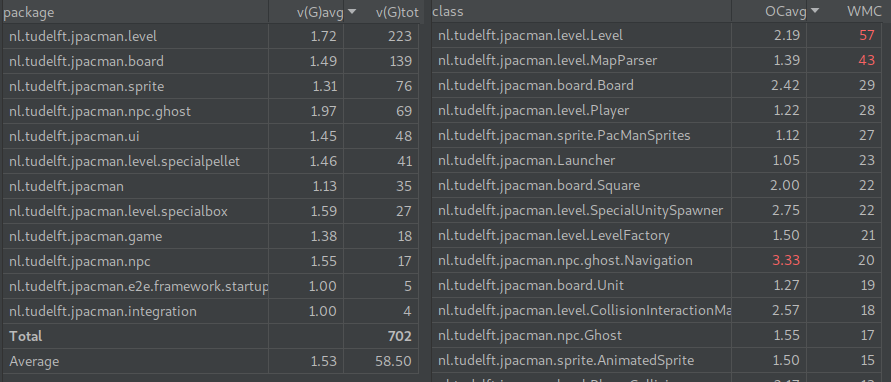
\includegraphics[width=\linewidth]{S1-compl_final}
\caption{Complexity metrics at package and class levels for final system 2}
\label{fig:S1_compl_final}
\end{figure}

\vspace{0.8cm}

The \wordlink{Figure}{fig:S1_depmatrix_final} confirms what Designite told us : the new written classes under \texttt{specialpellet} and \texttt{specialbox} packages didn't introduce new cycles in the system, preserving its design quality. There are still some big classes like \texttt{Level} implied in a lot of dependencies, but sometimes it's impossible to avoid it. \\

Another aspect is the javadoc coverage, that was initially very good. For the similar tabular than \wordlink{Figure}{fig:S1_javadoc_final}, we had in average 100\% (class coverage), 82\% (fields coverage), 232 lines of javadoc and 84\% (methods coverage). It looks like the documentation quality lowered, but we have to consider that the package structure changed. We also notice that the average number of lines increased, meaning that what had absolutly to be documented is well documented (some non relevant fields may have been omitted leading to the observed lowering).

\newpage

\vspace{0.2cm}

\begin{figure}[h]
\centering
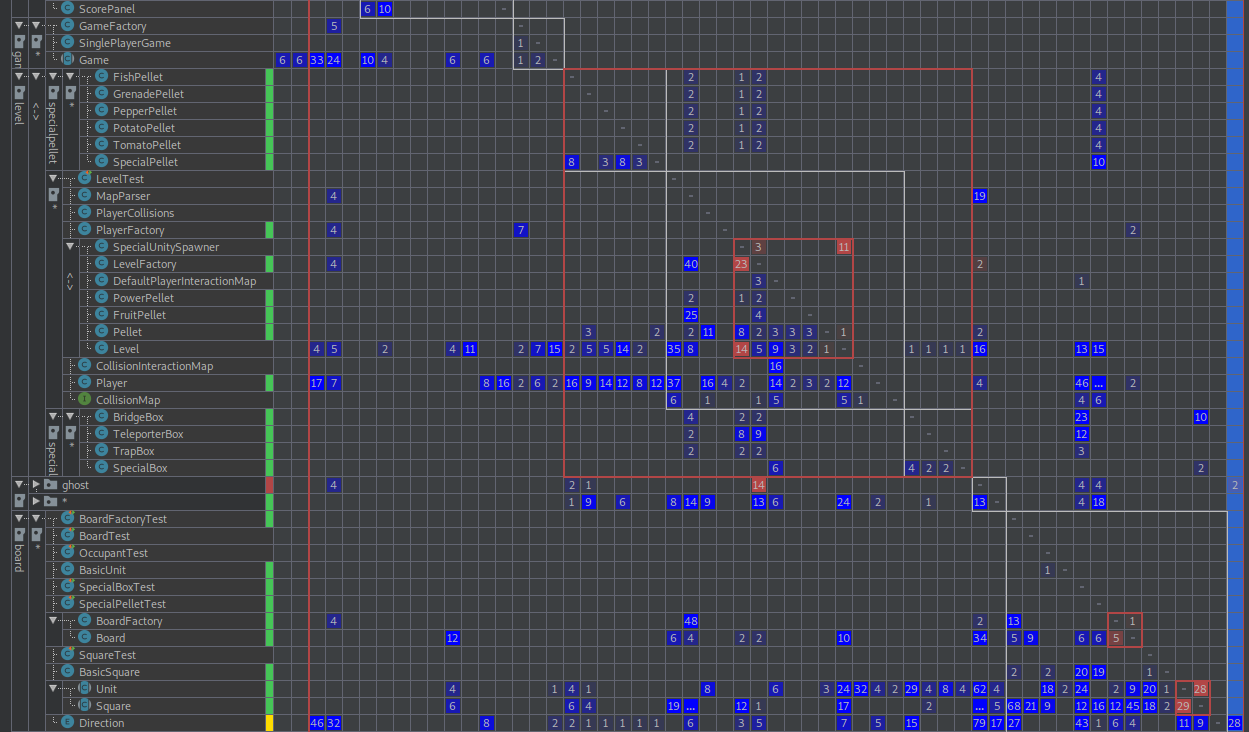
\includegraphics[width=0.95\linewidth]{S1-depmatrix_final}
\caption{Dependency matrix for final system 2}
\label{fig:S1_depmatrix_final}
\end{figure}

\vspace{0.3cm}

\begin{figure}[h]
\centering
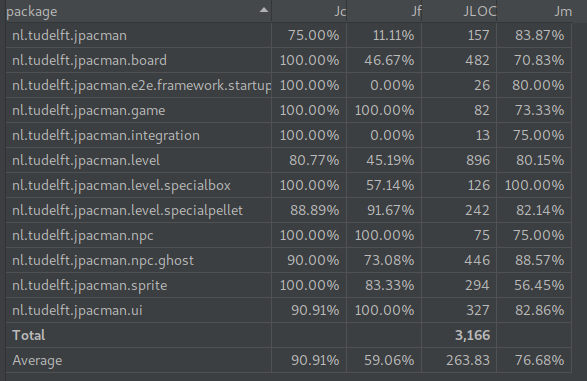
\includegraphics[width=0.52\linewidth]{S1-doc_final}
\caption{Results for javadoc coverage for final system 2}
\label{fig:S1_javadoc_final}
\end{figure}

\newpage

We use the test coverage provided by Intellij to analyze which part of the code are not under test coverage. Global results are given by \wordlink{Figure}{fig:S1_testcover_final}. We observe that the coverage stayed good, as new tests have been written to test the extension features. The 57 tests available (45 previously) pass without any problem.\\

\begin{figure}[h]
\centering
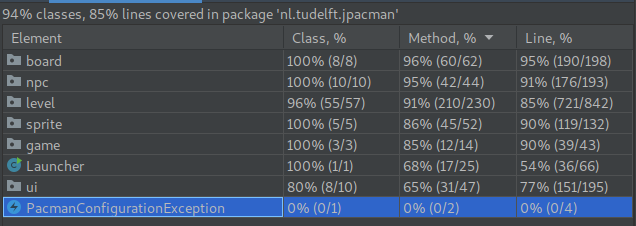
\includegraphics[width=0.8\linewidth]{S1-testcover_final}
\caption{Results for test coverage for final system 2}
\label{fig:S1_testcover_final}
\end{figure}

\section{Quality evolution analysis}
\newpage
\section{Conclusion}


\end{document}